\documentclass[a4paper,11pt,oneside]{book}

\usepackage[english]{babel}
\usepackage[showframe=false]{geometry}
\usepackage[usenames,dvipsnames]{xcolor}
\usepackage[utf8]{inputenc}
\usepackage[T1]{fontenc}
\usepackage{changepage}
\usepackage[]{algorithm2e}
\usepackage{amssymb}
\usepackage{amsmath}
\usepackage{graphicx}
\usepackage{listings}
\usepackage{verbatimbox}
\usepackage{ulem}
\usepackage{fancyvrb}
\usepackage{float}
\usepackage{hyperref}
\usepackage[parfill]{parskip}
\usepackage{tikz}
\usepackage{pdflscape}
\usepackage{minted}
\usepackage{titlesec}
\usepackage{titleps}
\usepackage{lastpage}
\usepackage{fancyhdr}
\usepackage{etoolbox}
\usepackage[]{algorithm2e}
%Following overwrites the page style for chapters
\patchcmd{\chapter}{\thispagestyle{plain}}{\thispagestyle{ruledChapter}}{}{}

%New page style for chapters
\newpagestyle{ruledChapter}{
	\setfoot{}{\thepage\ of \pageref{LastPage}}{}
	\footrule
	\renewcommand\makefootrule{\color{black}\rule[\baselineskip]{\linewidth}{0.4pt}}
}
%New page style for rest
\newpagestyle{ruled}{
	\sethead{\raggedright \chaptername\ \thechapter :\ \chaptertitle}{}{}
	\headrule
	\setfoot{}{\thepage\ of \pageref{LastPage}}{}
	\footrule
	\renewcommand\makeheadrule{\color{black}\rule[-.3\baselineskip]{\linewidth}{0.4pt}}
	\renewcommand\makefootrule{\color{black}\rule[\baselineskip]{\linewidth}{0.4pt}}
}

\expandafter\def\csname PY@tok@err\endcsname{}
\newcommand{\HRule}{\rule{\linewidth}{0.5mm}}
\newcommand{\specialcell}[2][c]{%
  \begin{tabular}[#1]{@{}c@{}}#2\end{tabular}}

\addtocontents{toc}{\protect\thispagestyle{empty}}

\title{}
\author{}
\date{} 

\begin{document}
\begin{titlepage}
\begin{center}

%-----------------------------------------------------------------
%							FRONTPAGE
%-----------------------------------------------------------------
\thispagestyle{empty}

\includegraphics[width=0.55\textwidth]{logo.pdf}\\[1cm]    
\textsc{\Large DM818 Assignment 3}\\[0.5cm]

% Title
\begin{Huge}
\textbf{DNS Algorithm}
\end{Huge}

\vspace{4cm}

% Author and supervisor
\begin{minipage}{1\textwidth}
\begin{center}
\emph{}\\

Dan \textsc{Sebastian Thrane}\\
\verb!<dathr12@student.sdu.dk>!\\

Lars \textsc{Thomasen}\\
\verb!<latho12@student.sdu.dk>!\\

\end{center}
\end{minipage}
\begin{minipage}{0.4\textwidth}
\end{minipage}

\vfill
% Bottom of the page
{\large Winter 2015}\\

\end{center}
\end{titlepage}

%-----------------------------------------------------------------
%							   TOC
%-----------------------------------------------------------------
\renewcommand{\contentsname}{Table of Contents}
\tableofcontents
\thispagestyle{empty}

%-----------------------------------------------------------------
%						  ACTUAL REPORT
%-----------------------------------------------------------------
\pagestyle{ruled}
\chapter{Introduction}
\setcounter{section}{1}
This report documents the development of an MPI virtual topology, and the implementation of the DNS algorithm covered in DM818.

The implementation takes some assumptions, such as it expects a cubic number $p$ of processors and assumes that the matrices of size $n*n \geq p^{1/3}$.

\section{Contributions}
Programming was done only using pair programming, and as such an equal contribution of this assignment has been done.

\chapter{Implementation}
\section{Design choices}
%A description of the design choices that you tried and how they affected the performance.
The implementation consists of two phases:
\begin{itemize}
\item Create virtual topology using MPI.
\item Follow the DNS algorithm.
\end{itemize}

Creating the virtual topology is a rather simple task, when a good understanding of how MPI works, and thus little to no design choices will be needed. 

While implementing the DNS algorithm, the design choices revolved around what type of communication calls to use.

Both of these are covered in the following sections.

\section{Virtual topologies}
%A description of how you used virtual topologies.
The communication pattern of a set of processes can be represented by a graph. The nodes in this graph is represented by processes and the edges between them is the processes communication between each other. MPI provides message-passing between any pair of processes in a group, often represented in a Communicator.

MPI offers built-in methods such as \verb!MPI_Graph_create! and \verb!MPI_Cart_create!. The latter offers the possibility to describe Cartesian structures in more than two dimensions.

The virtual topology was created in MPI using \verb!MPI_Cart_create!, this method takes the following parameters:
\begin{itemize}
\item MPI Communicator to which the Cartesian topology information is attached.
\item Number of dimensions.
\item Number of processes for each dimension.
\item Whether the dimensions are periodic.
\item Whether ranking may be reordered, if false the rank from the old communicator is retained.
\end{itemize}
and outputs a new communicator for the Cartesian topology. This is used to create a 3-dimension hypercube.

In order to communicate between the processes in this hybercube, we can create additional Communicators using \verb!MPI_Cart_sub!, specifying which dimensions we want our new communicator to attach to processes in. This helps simplifying the complexity of the communication code for the remaining part of the project.

As an example the following line specifies that we want all processes in the i'th axis in the new communicator \verb!iComm!.

\begin{verbatim}
int iDimensions[3] = {1, 0, 0};
MPI_Cart_sub(gridCommunicator, iDimensions, &iComm);
\end{verbatim}

Whenever we now want to communicate across all processes on the i'th dimension we can now simply use this communicator.

\section{The DNS algorithm}
Implementing the DNS algortihm can be divided into a few simple steps:
\begin{enumerate}
\item Distribute at k'th dimension.
\item Broadcast at j'th/i'th dimension.
\item Multiply.
\item Reduce k'th dimension to $k=0$.
\end{enumerate}

Initially the matrix is blocked and distributed among processes at the $k=0$ dimension. This distributing is done using \verb!MPI_Scatterv! which takes a vector of data and scatters it among the specified processes. Scatter was the correct choice here as each process in the k'th dimension requires each their data (a separate block of the matrix).

\begin{figure}[H]
  \centering
  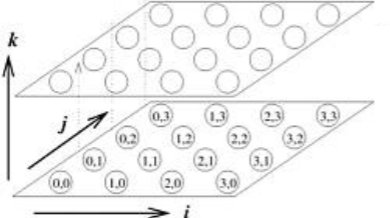
\includegraphics[width=0.5\linewidth]{dns1.jpg}
  \caption{Blocking and distribution of sub-matrices at k=0.}
  \centering
  \label{fig:sub1}
\end{figure}

\subsubsection*{Step 1: Distribute at k'th dimension}
% This needs a rewrite. But I doubt this will happen.
Following the algorithm from the book, the row \verb!j! is send to the k'th iteration. Such that $k=j$. This is done using Send for processes at $k=0$ and Receive for the processes at $k>0$. Using a single send and receive was chosen as this is a one-to-one communication, ie. a single process only has to hand their data to a single process at a higher dimension.

Note that this is the same procedure for the B matrix, just replace \verb!j! with \verb!i!.

\begin{figure}[H]
  \centering
  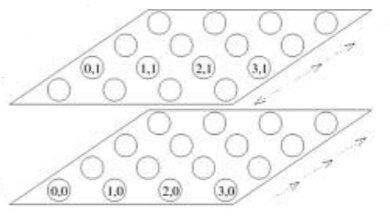
\includegraphics[width=0.5\linewidth]{dns2.jpg}
  \caption{Distribution from k=0 to k=j.}
  \centering
  \label{fig:sub1}
\end{figure}

\subsubsection*{Step 2: Broadcast at j'th dimension}
The data given to the dimensions at $k>0$ is then broadcasted to the processes along the j'th dimension. This is done using \verb!MPI_Bcast!, as we have a one-to-many communication, the previous process who received data has to transmit the same data to the remaining processes along j'th dimension.

Note that this is the same for the B matrix, using i'th dimension instead of j'th.

\begin{figure}[H]
  \centering
  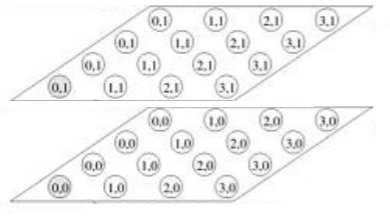
\includegraphics[width=0.5\linewidth]{dns3.jpg}
  \caption{Broadcast along j'th dimension}
  \centering
  \label{fig:sub1}
\end{figure}

\subsubsection*{Step 3: Multiply}
Simply multiplying matrix \verb!(i,j)! of A with matrix \verb!(j,i)! of matrix B. This is done using the naive implementation if run on Imada, or using the BLAS library if run on hopper. The result is stored in \verb!ResultMatrix! on each process.

\subsubsection*{Step 4: Reduce k'th dimension to $k=0$}
Reducing along the k'th dimension is done using \verb!MPI_Reduce!, since we are doing a many-to-one communication along the k'th dimension. All processes at $k>0$ sends their data to $k=0$. 

\section{Matrix not divisible by $p^{1/3}$}
%PADDING! TODO THIS SECTION!
In order to make it possible to run this algorithm on matrix sizes which is not divisible by $p^{1/3}$ we choose to apply padding.

Some background to understand this problem can be shown by thinking of the 3-dimensional cube split across p processes. Each dimension needs and equal amount of processes to split the n elements, if the $\frac{n}{p} != 0$ this will not be possible.

The simple solution is to pad the original matrix with additional elements with a value of 0. The end result will remain the same, at the cost of slight additional overhead multiplying and adding the 0's. The specific number of additional rows/columns added is calculated as following:

\begin{align*}
    \frac{n}{p^{1/3}} - n \mod p^{1/3}
\end{align*}

This calculates the number of elements per process first, and then subtracts the remainder we have. Thus we get the number of rows/columns we need.

\chapter{Performance}
\section{Runtimes}
%In your report, all runtimes and measures that depend on runtimes, should be based on average runtimes based on 10 test runs (compare main.c).

%Insert figure as Figure 5.8 and Table 5.1 in the book.
%1) As matrix-matrix multiplication with a small number of processors can take very long for large matrices, you 	should omit certain combination of p and n.
%2) HAVE to include (p,n) ∈ {(125,25),(125,10000),(1000,100),(1000,10000)} and a column for p=1. 

%A table with the same columns and rows as the table given above, where the entries should give the percentage  	of the overall runtime that was spend for computation (use MPI_Wtime for measuring computation times between communication periods on one node only).

%A table with the same columns and rows as the table given above, where the entries should give the overall runtime in seconds (use MPI_Wtime for measuring computation times between communication periods on one node only).

\chapter{Isoefficiency of the implementation}
%A discussion of your results and a discussion that compares your results to the isoefficiency function O(p(log p)^3).
Need the results first.

\chapter{Testing}
%Your source code has to include a method that checks for a randomly chosen element of the resulting matrix, that the outcome of the parallel matrix multiplication is identical to the result that is computed in O(n) time on one node (that is the difference is smaller that a reasonably chosen small value). The correctness check should not influence the overall runtime measurements. Your executable has to perform the correctness check on at least one element.
Confirming that the final results are correct have been verified in two methods:

\begin{itemize}
\item Manually
\item Random element check each iteration
\end{itemize}

The former was done using small numbers of \verb!n!, this was initially done to verify that the algorithm atleast works correctly.

The latter will each iteration calculate the matrix multiplication on the root process, and then pick a random element and compare it against the two matrices. This is done using and assert, which would halt the program if not held. An error tolerance of 0.001 was put in place to allow for rounding errors.
This testing is done after saving the \verb!endtime!, thus the overall runtime measurements are not affected.

\chapter{Conclusion}
Compared to the previous assignment, less time was spent on understanding how MPI works. Instead the challenge was understanding how to build Cartesian structures. This builds nicely on-top of what we previous learned and in the end gave a fundamentally understanding how to work within a parallel environment using MPI.

The DNS algorithm itself was rather simple, the biggest issue was getting ones head around how to do the communication between the processes correctly.

A working program was somewhat quickly composed (compared to the previous assignment) after spending a fair amount of time discussing how to attack the problem correctly. Due to severe lack of time, the code has not been adhered to different coding standards, and should be re-factored if ever worked with again.


%-----------------------------------------------------------------
%						     APPENDIX
%-----------------------------------------------------------------
%/newpage
%\newgeometry{left=2.5cm,right=2.5cm}
%\chapter{Appendix}
%\section{Serial algorithm plotting data}

\end{document}
